\chapter{Process Perspective}

\section{Developer Interaction}

During the development process, the majority of interaction among the developers has occurred on-site. The group has met one to two times per week to collaboratively develop new features, while smaller ad hoc tasks have been solved individually. Communication in remote contexts has been facilitated by the use of Discord and Facebook Messenger. All documentation such as a guide for local env. setup, release notes, money spent and code guidelines have been manually written and shared on Notion. 

\section{Team Organisation}

The organization of the team and distribution of tasks have represented an important aspect of the project's success, considering that each developer attends different courses and jobs which can disrupt communication. To address this challenge, the group has used GitHub Issues, which allows for the creation of a Kanban board displaying pending tasks, their respective type, and current progress. By doing so, the group has been able to maintain transparency of work progress without relying on constant communication.

\section{CI/CD}
\label{sec:ci-cd}

To facilitate the Continues Integration of new code by all developers, several workflows/pipelines have been implemented to ensure that each pull request (\texttt{PR}) is subjected to checks and analyses, including building, testing, and code scanning to mitigate the risk of the service breaking. Once these checks are successfully completed, the \texttt{PR} is deemed safe for merging into the main branch, which initiates a deployment pipeline. The following subsections give a brief explanation of each workflow. 

\subsection{\texttt{build-test.yml}}

This workflow performs the build and testing of the stack in the service, including the backend and frontend. The pipeline is triggered on push events to any branch and includes two jobs: \\

\textbf{build-test-backend}, which runs on an Ubuntu 20.04 machine and includes the following steps:

\begin{enumerate}
    \item Checkout the repository
    \item Set up .NET version 7.0.x
    \item Restore dependencies
    \item Build the \texttt{MiniTwit} backend
    \item Run backend tests
\end{enumerate}

\textbf{build-test-frontend}, which runs on an Ubuntu 22.04 machine and includes the following steps:

\begin{enumerate}
    \item Checkout the repository
    \item Install \texttt{Node.js} version 18 and dependencies for caching
    \item Install dependencies for the \texttt{MiniTwit} frontend
    \item Build the \texttt{MiniTwit} frontend
    \item Run frontend tests using \texttt{Playwright}, in a docker container started by \texttt{docker-compose -f docker-compose.ui.yml up -d}
    \item Stop the UI service by shutting down the Docker containers created with docker-compose
\end{enumerate}

\subsection{\texttt{eslint.yml}}

A pipeline that integrates \textit{eslint} for checking the frontend code. This workflow automatically detects and reports issues in the code by uploading a \textit{.sarif} file to GitHub. It provides guidance on how to fix the issues reported, such as unused variables, unused imports, and type-related errors. 

\begin{figure}[H]
    \centering
    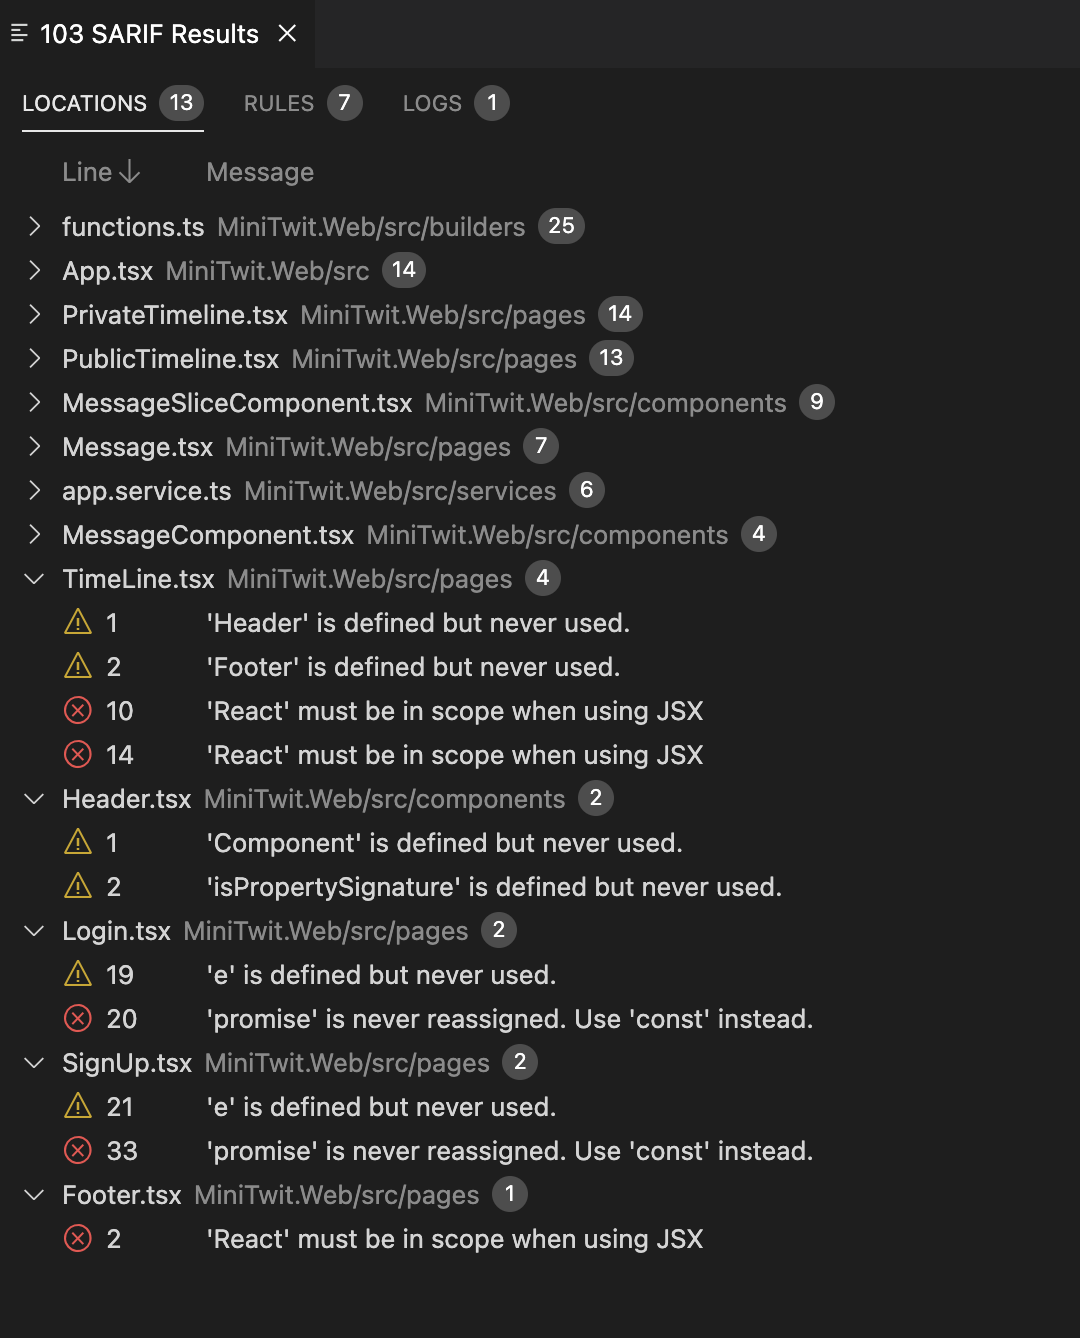
\includegraphics[width=10cm]{Eslint_report.png}
    \caption{Eslint scan - Report.}
    \label{fig:elsint_report}
\end{figure}

\subsection{\texttt{codeql.yml}}

A pipeline that integrates \texttt{CodeQL} (C\# analysis), which scans the backend code for C\# specific vulnerabilities and bugs. It also provides guidance on how to fix them.

\subsection{\texttt{snyk-security.yml}}

A pipeline that integrates with \texttt{Snyk}, which provides continuous security monitoring. The pipeline scans the project's dependencies to identify any known vulnerabilities and automatically sets up a \texttt{PR} that updates outdated packages or packages containing known vulnerabilities. 

\begin{figure}[H]
    \centering
    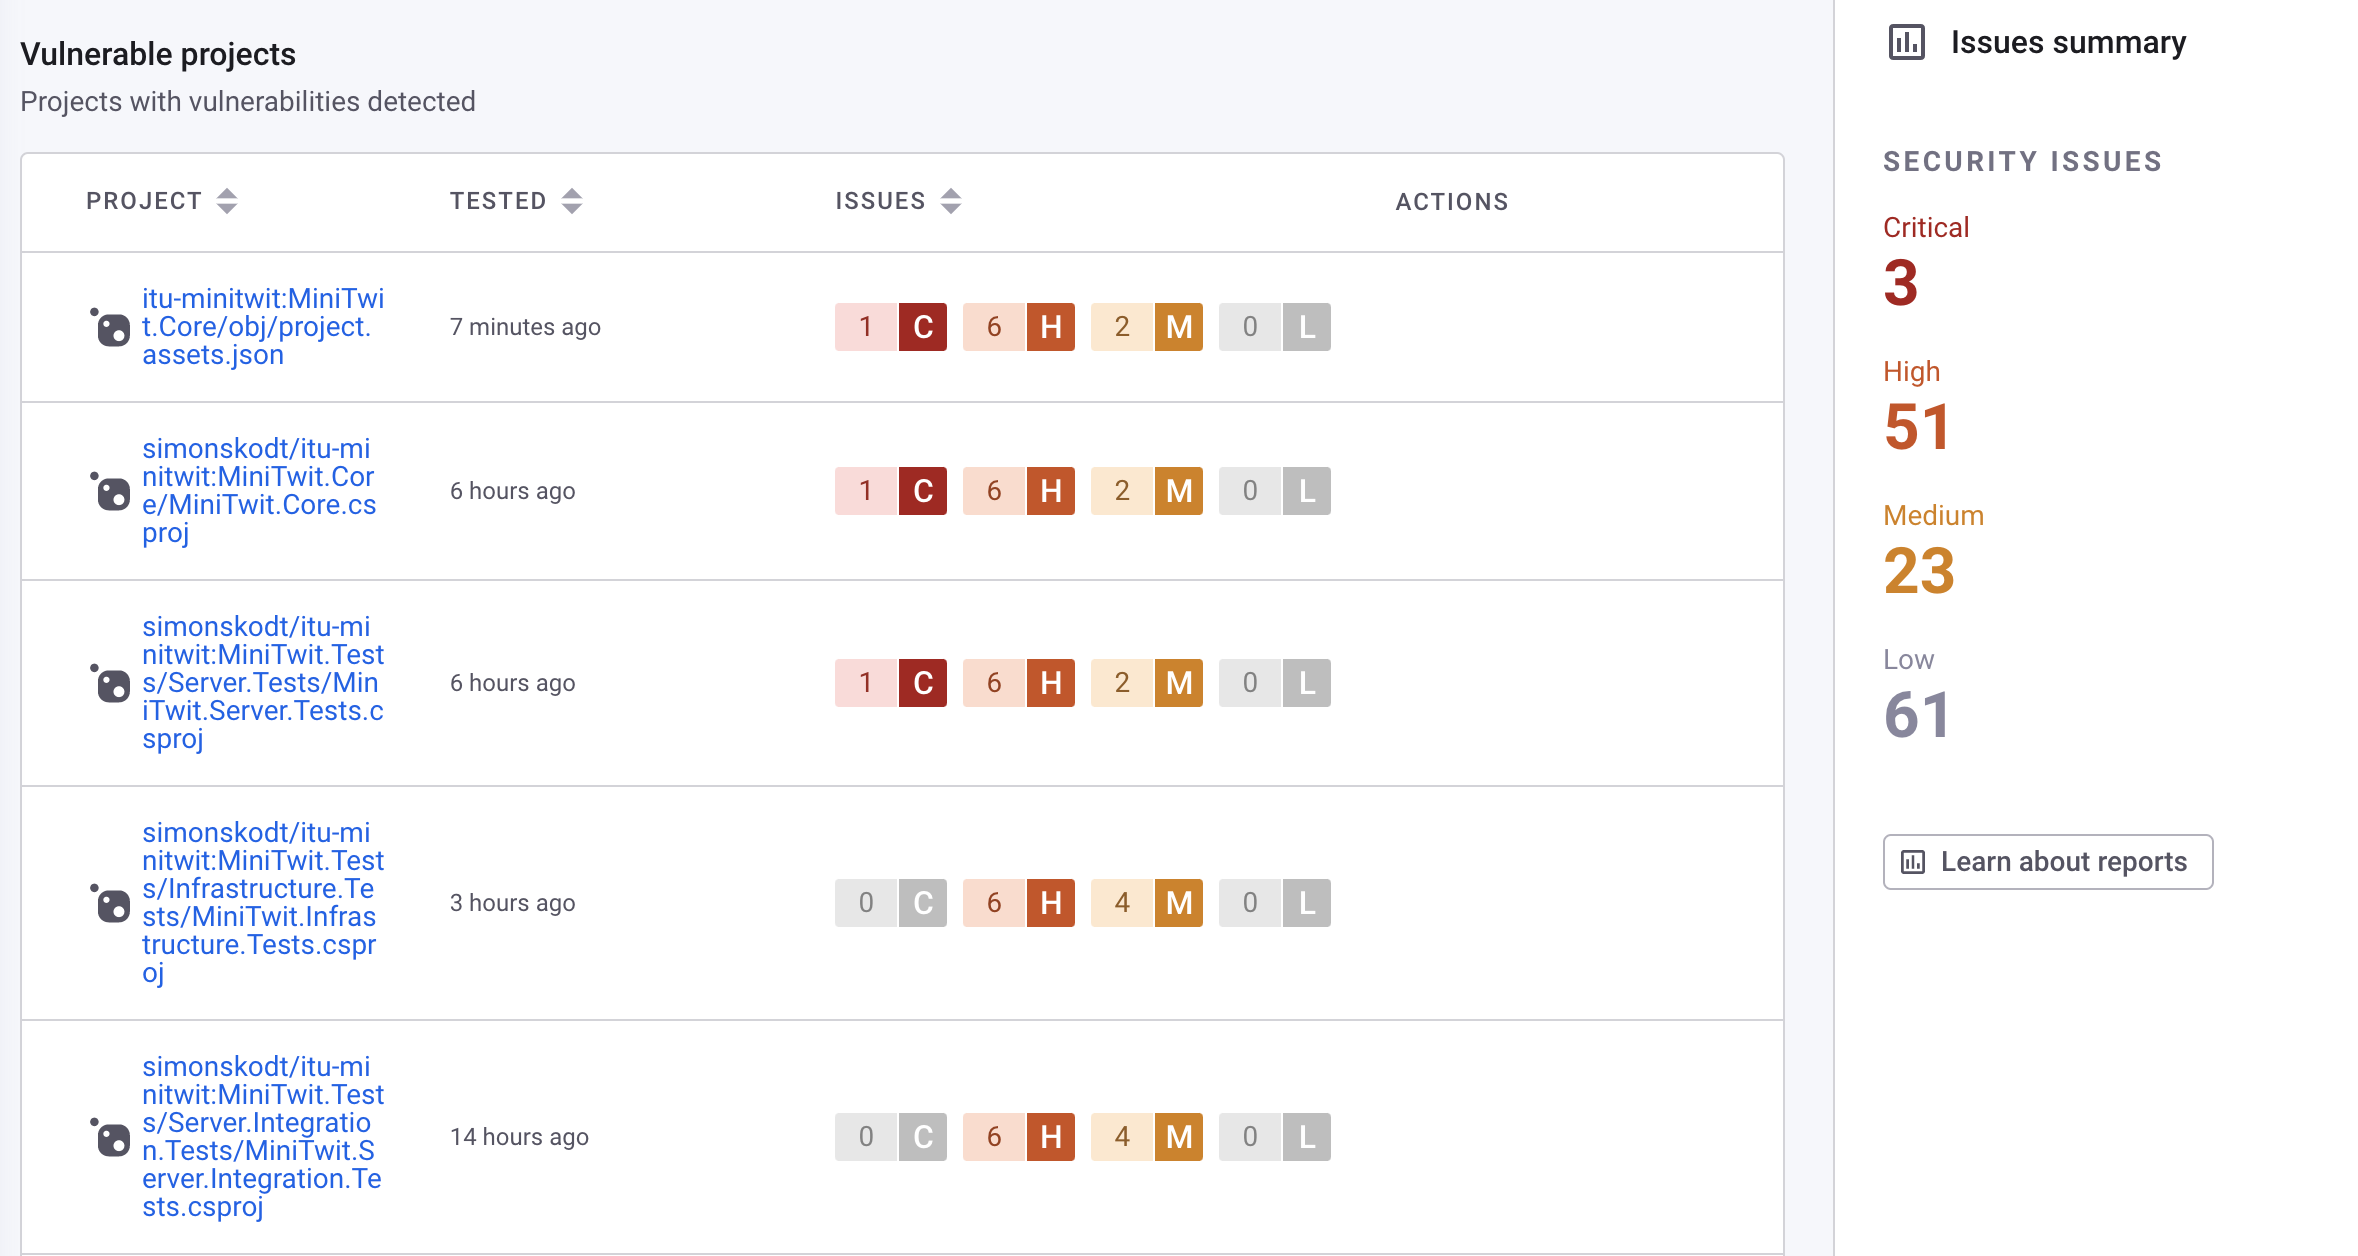
\includegraphics[width=14cm]{Snyk_report.png}
    \caption{\textit{Snyk} Security --- report.}
    \label{fig:snyk_report}
\end{figure}

\subsection{\texttt{continuous-deployment.yml}}

All pipelines highlighted so far, are triggered either by pushing to a development branch or creating a \texttt{PR} to the main branch. The combination of these pipelines constitutes the project's \textit{deployment gate} which is a collection of predefined checks and signals that must pass before a deployment may be triggered \cite{DevOps_gates}. If the \texttt{PR} passes the gate, it can be deployed. This is done by merging the \texttt{PR}, which will trigger the continuous-deployment pipeline.

The continuous-deployment pipeline is separated into two jobs, namely build and deploy. The \textit{build} job is responsible for building and pushing the Docker images for the \texttt{MiniTwit} backend and frontend, respectively. The job uses the Docker Build tool to build the images and then pushes them to Docker Hub.

The \textit{deploy} job is responsible for deploying the \texttt{MiniTwit} application and monitoring/logging components to the live server. This job is dependent on the \textit{build} job to ensure that the images are built and available for deployment. The job first uses the \textit{rsync} command to copy the Docker Compose files and monitoring/logging configuration files to the live server. It then uses the SSH Action to log in to the live server and deploys the \texttt{MiniTwit} application and monitoring/logging components by executing the docker-compose files: \textit{docker-compose.prod.yml} and \textit{docker-compose.monitoring.yml}.

\section{Repository Organisation}

The group has employed a mono-repository approach, in which all components are stored within a single GitHub repository. While the option to maintain separate repositories for the frontend and backend existed, it was decided that, given the size of this project, a mono-repository was better with regards to the standardization of branch strategies, review of pull requests, and deployment strategy, i.e. we can deploy the whole service from a single \texttt{PR}.

\section{Branching Strategy}

We have used a trunk-based branching strategy where we work with two types of branches.

\begin{itemize}
    \item The main branch/trunk branch (long-lived)
    \item Several feature branches (short-lived)
\end{itemize}

The main branch always contains the newest working instance of \texttt{MiniTwit}. The feature branches are short-lived branches containing new features for \texttt{MiniTwit}. As soon as a feature is completed, the feature branch is merged with the main branch using pull requests. Once the merge is accomplished, the feature branch is deleted. Due to branch protection rules merge request can only be accepted onto the main branch after it has undergone review, approval, and has passed all pipeline checks. In order to maintain a clean history of the version control system, it is recommended that each branch correspond to an issue on GitHub, and that commit messages have the following format:

\begin{verbatim}
    <commit type>([scope]): <message>
\end{verbatim}

\section{Monotoring}

When it comes to monitoring \texttt{MiniTwit}, we only monitor the backend. For this, we use \texttt{Prometheus} by importing the \texttt{Prometheus} NuGet package in the \texttt{Presentation Layer}. Out of the box \texttt{Prometheus} provides a \texttt{/metrics} endpoint to scrape for the following metrics:

\begin{itemize}
    \item Whether \texttt{Prometheus} and the backend is up
    \item Requests per controller per endpoint
    \item Total number of requests
    \item Average request response time
    \item CPU usage
    \item Memory usage
    \item Number of requests with successful and unsuccessful response code
\end{itemize}

\texttt{Prometheus} is scraped by \texttt{Grafana} and the metrics are visualized in our monitoring dashboard, which can be seen in figure \ref{fig:Minitwit_logging}. The dashboard visualizes the information about the average response time, number of requests, etc. which has been useful to detect any abnormalities in the project. Especially the average response time, which in the beginning was way too high for the system to work properly when multiple incoming requests were handled.

\begin{figure}[H]
    \centering
    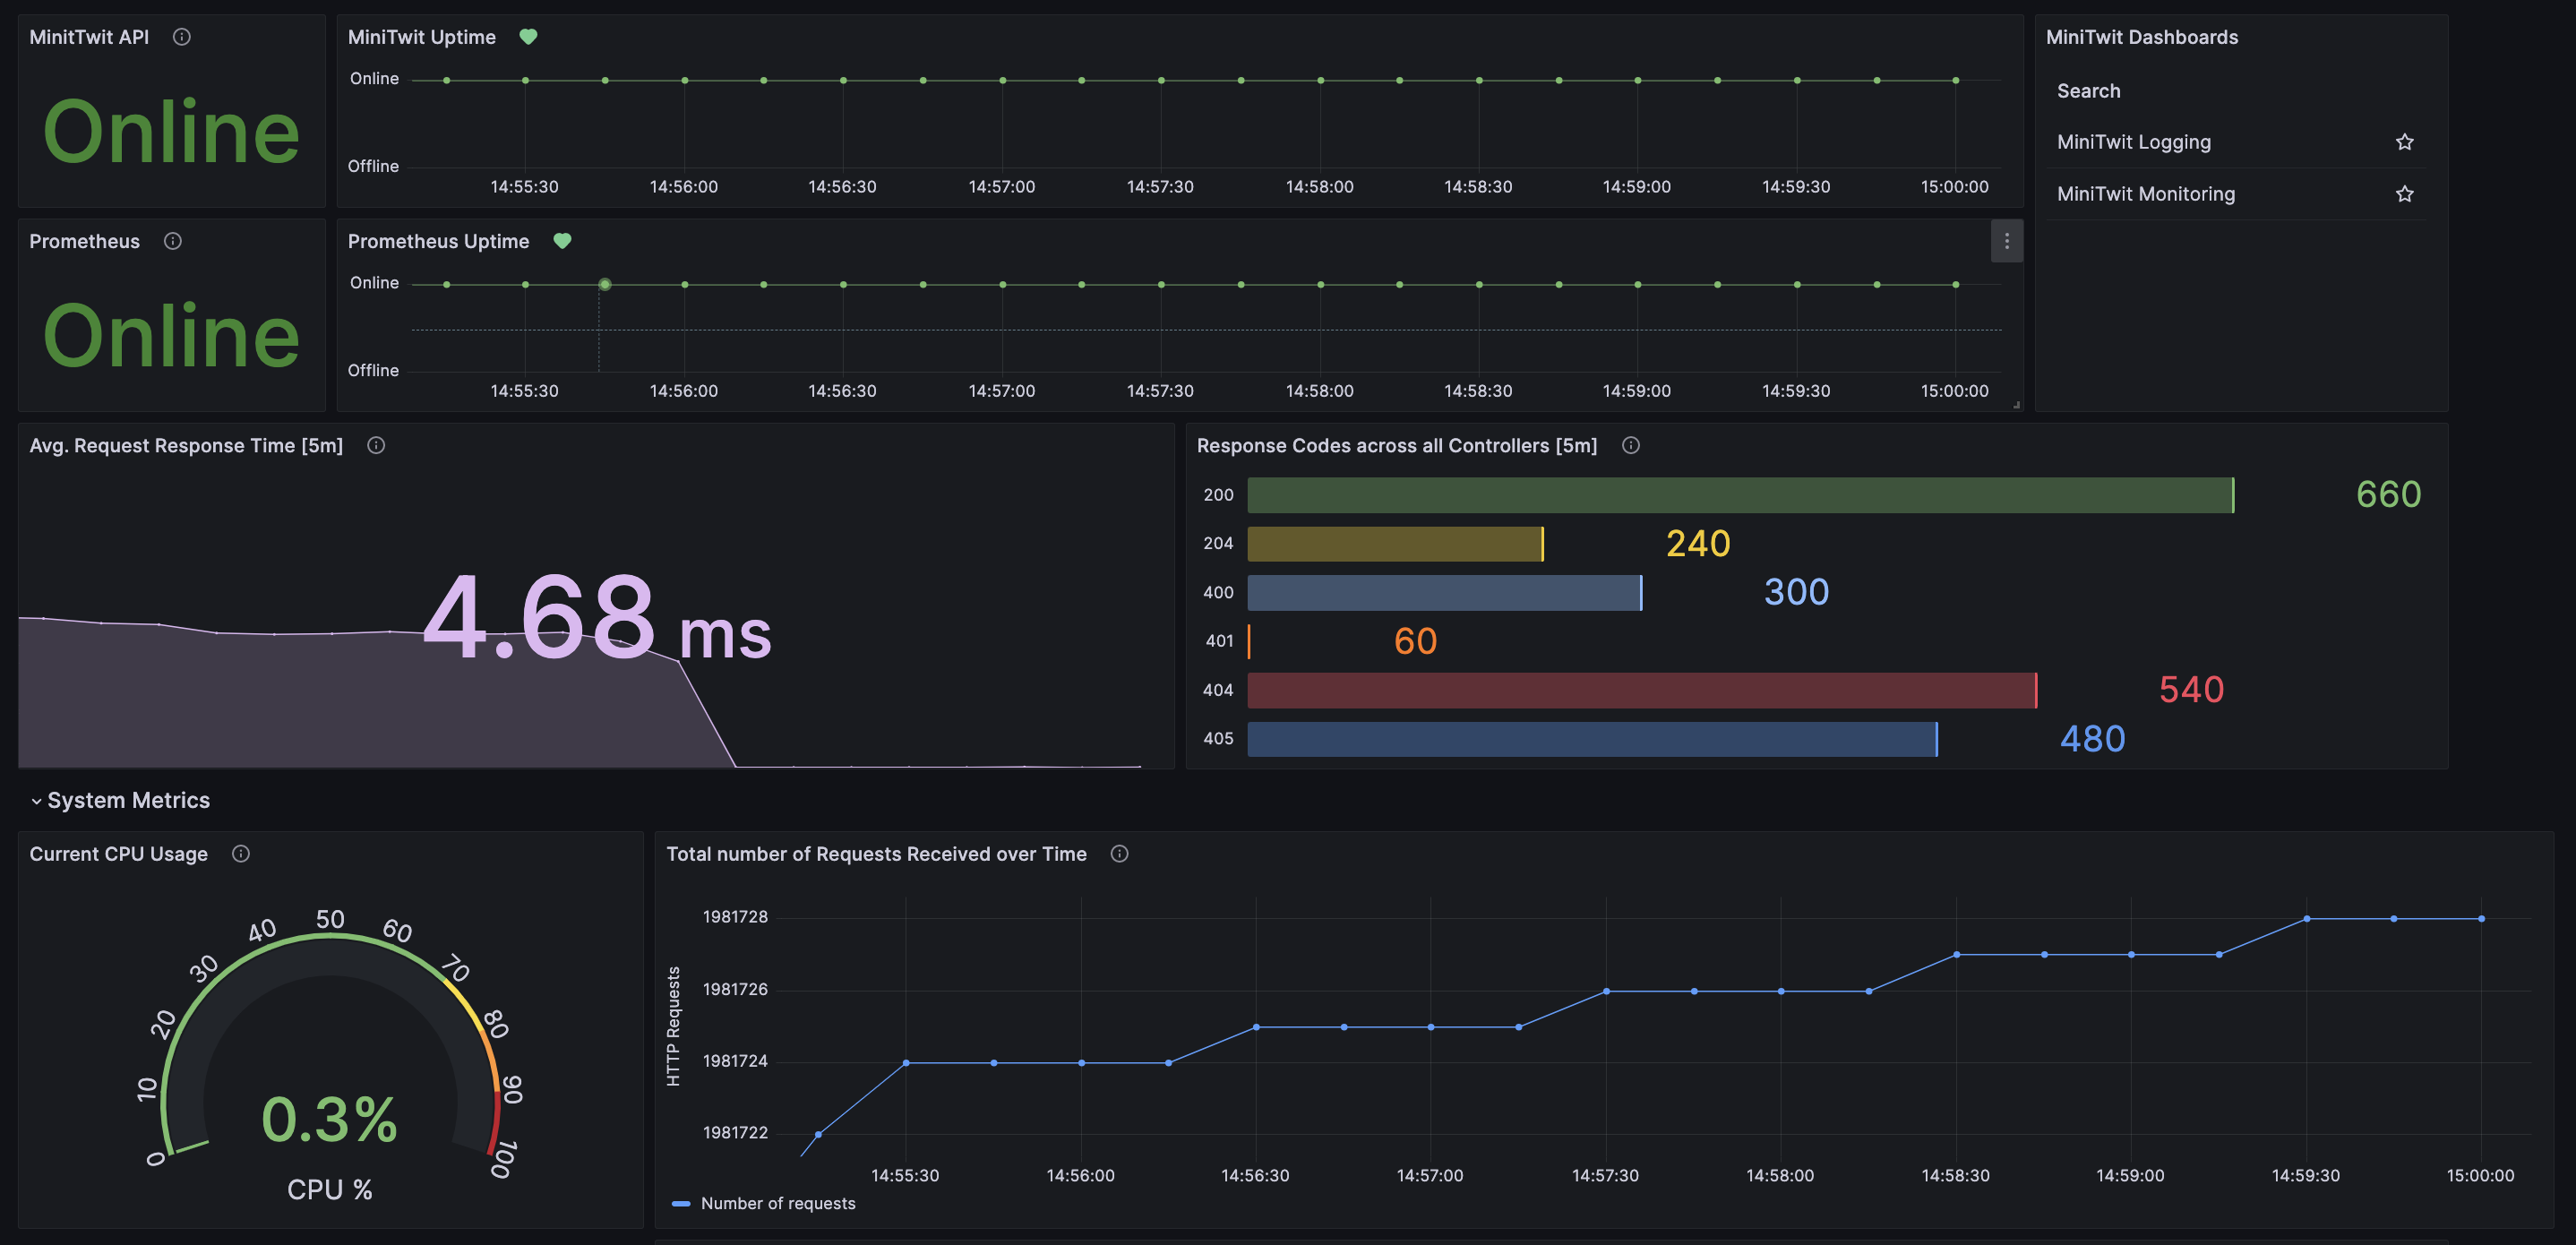
\includegraphics[width=\linewidth]{Monitoring.png}
    \caption{\texttt{Grafana} monitoring dashboard for monitoring the \texttt{MiniTwit} backend.}
    \label{fig:Minitwit_monitoring}
\end{figure}

\section{Logging}

For logging the \texttt{MiniTwit} backend, we used \texttt{Loki}. We use \texttt{Loki} by importing the \texttt{Loki} NuGet package. When logging, \texttt{Loki} automatically sends the logs to a running \texttt{Loki} server instance which is directly queried by \texttt{Grafana}. We only log within the \texttt{Presentation Layer} in the two controllers. The log level used when logging depends on the response state from the service layer, specifically, we use:

\begin{itemize}
    \item \textbf{Error:} When the \texttt{Service Layer} returns errors when usernames or ids are not found.
    \item \textbf{Warning:} When an unexpected status is returned from the \texttt{Service Layer}.
    \item \textbf{Information:} When a request is successfully executed, describe what happened.
    \item \textbf{Debug:} When we want to debug information such as the number of Tweets fetched from the backend etc.
\end{itemize}

\begin{sidewaysfigure}[H]
    \centering
    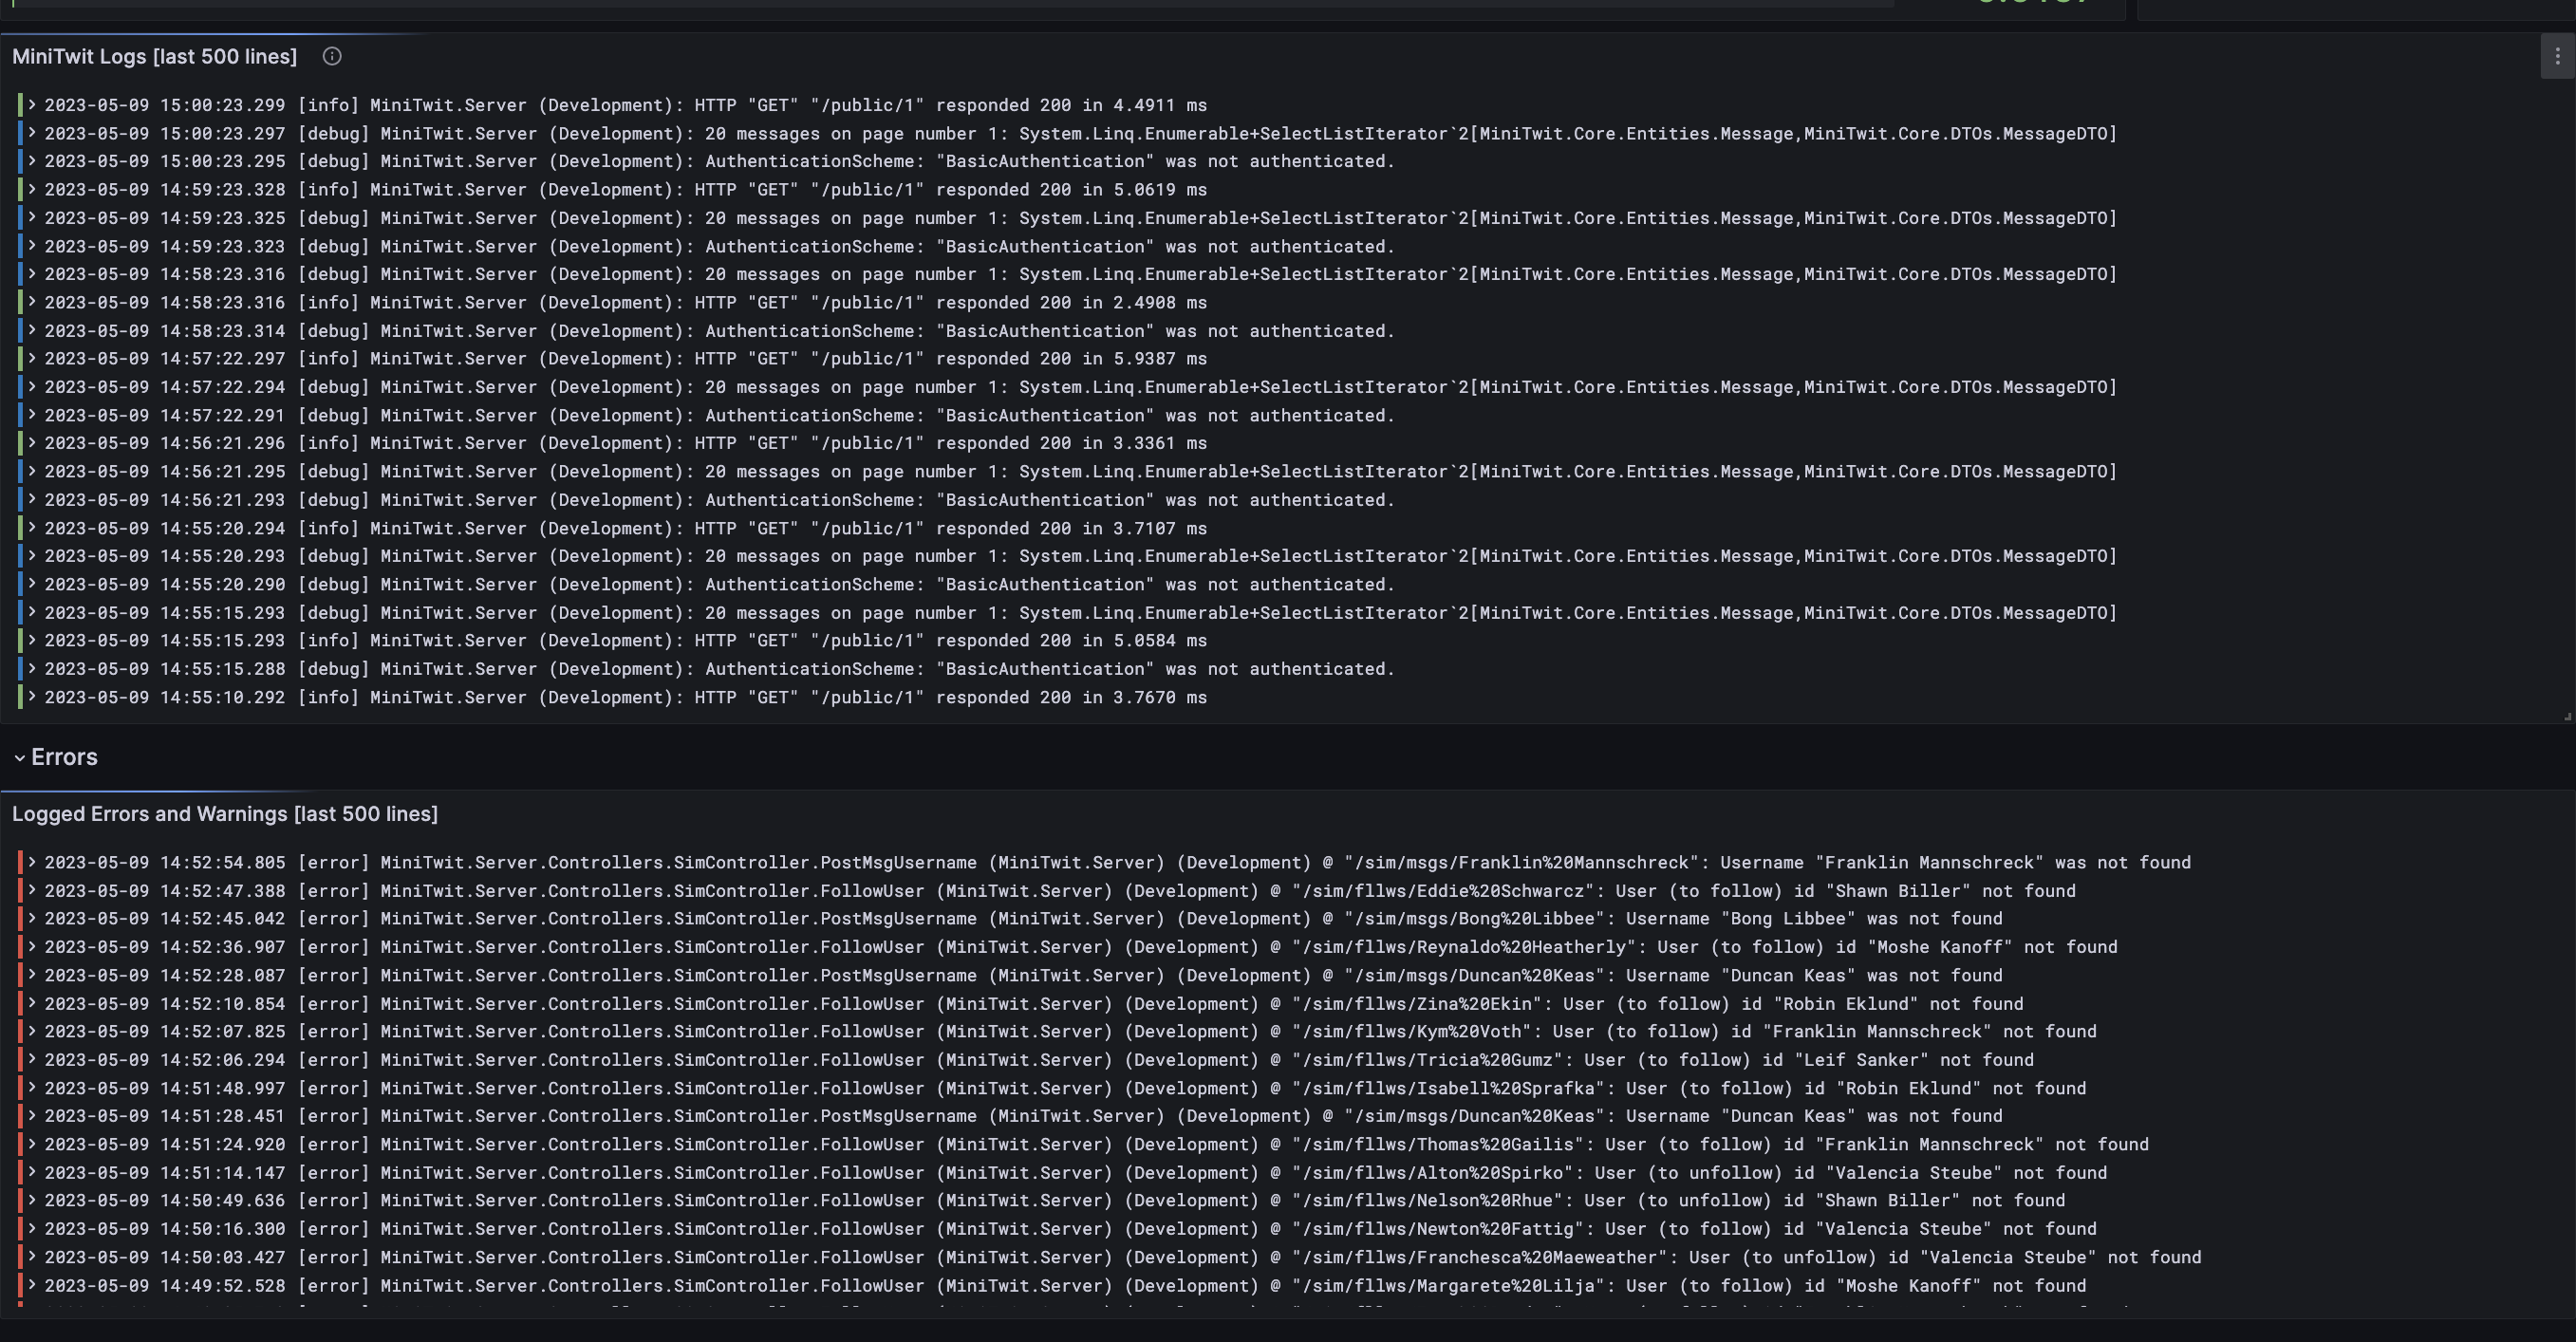
\includegraphics[width=\linewidth]{Logging.png}
    \caption{Logging from our \texttt{Grafana} logging dashboard.}
    \label{fig:Minitwit_logging}
\end{sidewaysfigure}

\section{Security}

As seen in the following security assessment: \href{https://github.com/simonskodt/itu-minitwit/blob/main/Documents/SECURITY_ASSESSMENT.md}{\textit{secuirty assesment}}, we found that our service lacked security measurements, particularly the absence of TLS configuration. To address this issue, the team attempted to implement TLS using \texttt{NGINX} and \texttt{Certbot}, aiming to secure the obtained domain "\underline{https://minitwit.live/}". However, we encountered difficulties in obtaining a certificate, likely caused by the server's firewall blocking the request to \texttt{Certbot}.

\section{Scaling and Load Balancing}

In terms of scaling, we created a Docker Swarm for horizontal scaling, following the instructions provided during the lecture.  The swarm was successfully set up, and it functioned as intended in theory. However, we never fully understood how the setup communicated between the machines, particularly the mapping of frontends to corresponding backends. Although we had three instances of our service running within the swarm, we were hesitant to replace our production droplet with the swarm due to our lack of confidence in operating and maintaining it effectively. 

The setup was created by the following shell script \href{https://github.com/simonskodt/itu-minitwit/blob/feat-swarm/swarm.sh
}{swarm.sh}, which served as our implementation of Infrastructure as Code. Scripts were not employed for creating virtual machines (VMs) beyond this point, as we found the \textit{DigitalOcean} user interface to be very intuitive. Nevertheless, we acknowledge the importance of employing tools such as \textit{Vagrant} or \textit{Terraform} for VM creation, as they would simplify a handover of the project.

\section{Use of Artificial Intelligence} 

This project utilized ChatGPT to solve specific code issues. Additionally, AI has been used to grammatically correct sentences. However, the AI's suggestions were not blindly copied, as the essence of the sentences could be lost in the process.
